\documentclass[border=4pt]{standalone}
\usepackage{tikz}
\usepackage{fontspec}
\usepackage{amsmath}
\usetikzlibrary{arrows.meta,positioning}
\setmainfont{SpaceGrotesk}[Path=fonts/,Extension=.ttf,UprightFont=*-400,BoldFont=*-700,FontFace={md}{n}{*-500}]
\setsansfont{SpaceGrotesk}[Path=fonts/,Extension=.ttf,UprightFont=*-400,BoldFont=*-700]
\renewcommand{\familydefault}{\sfdefault}
\definecolor{teal}{HTML}{1F6F86}
\definecolor{amber}{HTML}{C8881E}
\definecolor{accent}{HTML}{157E6B}
\definecolor{ink}{HTML}{15171C}
\definecolor{muted}{HTML}{5C616B}
\begin{document}
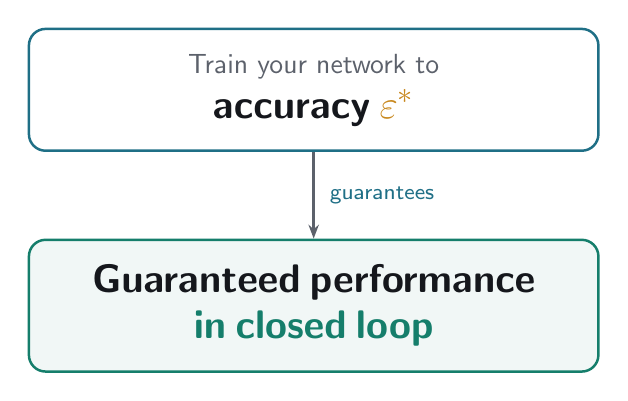
\begin{tikzpicture}[font=\sffamily]
  \node[draw=teal, line width=0.9pt, rounded corners=6pt, inner sep=9pt, text width=66mm, align=center] (a)
    {{\color{muted}\fontsize{10}{12}\selectfont Train your network to}\\[3pt]
     {\color{ink}\fontsize{15}{17}\bfseries accuracy {\color{amber}$\varepsilon^{*}$}}};
  \node[below=11mm of a, draw=accent, line width=0.9pt, rounded corners=6pt, fill=accent!6,
        inner sep=9pt, text width=66mm, align=center] (b)
    {{\color{ink}\fontsize{14}{16}\bfseries Guaranteed performance}\\[3pt]
     {\color{accent}\fontsize{14}{16}\bfseries in closed loop}};
  \draw[-{Stealth[length=5pt]}, muted, line width=1pt] (a) -- (b)
    node[midway, right=2pt, text=teal, font=\fontsize{8.5}{10}\selectfont] {guarantees};
\end{tikzpicture}
\end{document}
